%
% This is a borrowed LaTeX template file for lecture notes for CS267,
% Applications of Parallel Computing, UCBerkeley EECS Department.
% Now being used for CMU's 10725 Fall 2012 Optimization course
% taught by Geoff Gordon and Ryan Tibshirani.  When preparing 
% LaTeX notes for this class, please use this template.
%
% To familiarize yourself with this template, the body contains
% some examples of its use.  Look them over.  Then you can
% run LaTeX on this file.  After you have LaTeXed this file then
% you can look over the result either by printing it out with
% dvips or using xdvi. "pdflatex template.tex" should also work.
%

\documentclass[twoside]{article}
\setlength{\oddsidemargin}{0.25 in}
\setlength{\evensidemargin}{-0.25 in}
\setlength{\topmargin}{-0.6 in}
\setlength{\textwidth}{6.5 in}
\setlength{\textheight}{8.5 in}
\setlength{\headsep}{0.75 in}
\setlength{\parindent}{0 in}
\setlength{\parskip}{0.1 in}

%
% ADD PACKAGES here:
%

\usepackage{amsmath,amsfonts,graphicx}

%
% The following commands set up the lecnum (lecture number)
% counter and make various numbering schemes work relative
% to the lecture number.
%
\newcounter{lecnum}
\renewcommand{\thepage}{\thelecnum-\arabic{page}}
\renewcommand{\thesection}{\thelecnum.\arabic{section}}
\renewcommand{\theequation}{\thelecnum.\arabic{equation}}
\renewcommand{\thefigure}{\thelecnum.\arabic{figure}}
\renewcommand{\thetable}{\thelecnum.\arabic{table}}

%
% The following macro is used to generate the header.
%
\newcommand{\lecture}[4]{
   \pagestyle{myheadings}
   \thispagestyle{plain}
   \newpage
   \setcounter{lecnum}{#1}
   \setcounter{page}{1}
   \noindent
   \begin{center}
   \framebox{
      \vbox{\vspace{2mm}
    \hbox to 6.28in { {\bf EE402 - Discrete Time Systems
	\hfill Spring 2018} }
       \vspace{4mm}
       \hbox to 6.28in { {\Large \hfill Lecture #1 \hfill} }
       \vspace{2mm}
       \hbox to 6.28in { {\it Lecturer: #2 \hfill } }
      \vspace{2mm}}
   }
   \end{center}
   \markboth{Lecture #1}{Lecture #1}

   \vspace*{4mm}
}
%
% Convention for citations is authors' initials followed by the year.
% For example, to cite a paper by Leighton and Maggs you would type
% \cite{LM89}, and to cite a paper by Strassen you would type \cite{S69}.
% (To avoid bibliography problems, for now we redefine the \cite command.)
% Also commands that create a suitable format for the reference list.
\renewcommand{\cite}[1]{[#1]}
\def\beginrefs{\begin{list}%
        {[\arabic{equation}]}{\usecounter{equation}
         \setlength{\leftmargin}{2.0truecm}\setlength{\labelsep}{0.4truecm}%
         \setlength{\labelwidth}{1.6truecm}}}
\def\endrefs{\end{list}}
\def\bibentry#1{\item[\hbox{[#1]}]}

%Use this command for a figure; it puts a figure in wherever you want it.
%usage: \fig{NUMBER}{SPACE-IN-INCHES}{CAPTION}
\newcommand{\fig}[3]{
			\vspace{#2}
			\begin{center}
			Figure \thelecnum.#1:~#3
			\end{center}
	}
% Use these for theorems, lemmas, proofs, etc.
\newtheorem{theorem}{Theorem}[lecnum]
\newtheorem{lemma}[theorem]{Lemma}
\newtheorem{proposition}[theorem]{Proposition}
\newtheorem{claim}[theorem]{Claim}
\newtheorem{corollary}[theorem]{Corollary}
\newtheorem{definition}[theorem]{Definition}
\newenvironment{proof}{{\bf Proof:}}{\hfill\rule{2mm}{2mm}}

% **** IF YOU WANT TO DEFINE ADDITIONAL MACROS FOR YOURSELF, PUT THEM HERE:

\begin{document}

% Lecture Details
\lecture{4}{Asst. Prof. M. Mert Ankarali}

\par

\section*{Realization of Discrete Time Systems / Filters / Controllers}

This lecture will cover some fundamental block-diagram realization
techniques for discrete-time systems, filters, \& controllers represented by Z-Domain transfer functions or difference equations.

Block-diagram realizations are extremely useful practically to implement the system/filter/controller on a physical embedded platform. Whether your goal is to programming the discrete filter/controller on a microcontroller or embedding the structure on a FPGA module, a block diagram representation is always helpful.

In the last phase of the course, we will also actively use 
block-diagram representation to obtain a state-space realization
from a given discrete-time system.

The most fundamental block for a discrete-time system is the unit
delay operator 
%
\begin{align*}
y[k] &= x[k-1] \\ 
Y(z) &= z^{-1} X(z)
\end{align*}
%
which is represented by the following block-diagram 
%
\begin{center}
  \begin{minipage}[h]{0.9\linewidth}
    \begin{center}
      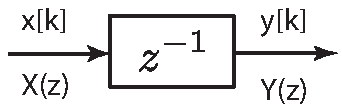
\includegraphics[width=0.3\textwidth]{delay}
    \end{center}
  \end{minipage}
\end{center}
%
In this lecture, our goal is to realize different kinds of
discrete-time transfer functions using this fundamental
block as the main brick.

\newpage

\subsection*{Realization of FIR Systems}

A third order (order is fixed for the sake of clarity) FIR (Finite
impulse response) discrete time system has the following
difference equation and transfer function
%
\begin{align*}
y[k] &= b_0 x[k] + b_1 x[k-1] + b_2 x[k-2] + b_3 x[k-3] \\ 
Y(z) &= \left( b_0 + b_1 z^{-1} + b_2 z^{-2} + b_3 z^{-3} \right) X(z)
\end{align*}
%
From inspection it is easy to see that we need at least three unit delay 
blocks (and memory elements) to construct a full realization. Below the
block-diagram realization of a third order FIR is given in Fig.~\ref{fig:FIR}
%
\begin{figure}[h]
    \centering
      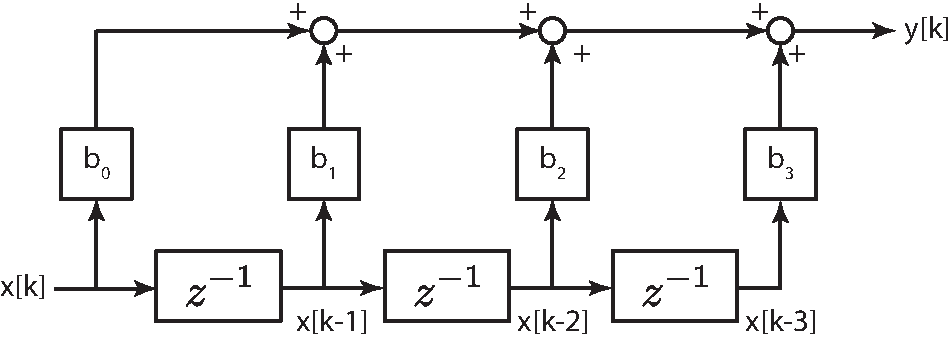
\includegraphics[width=0.9\textwidth]{FIR}
    \caption{Block diagram realization of a third order FIR system}
        \label{fig:FIR}
\end{figure}

\newpage

\subsection*{Realization of IIR Systems with Static Numerator Dynamics}
%
In this part we will analyze a special case if IIR (Infinite impulse
response) systems where the input dynamics is static, i.e. there is no 
direct delayed term of the input in the difference equation. Again for
the sake of clarity let's assume that the discrete system is third
order. For such a system, the difference equation and the transfer
function can be written as
%
\begin{align*}
y[k] &= -a_1 y[k-1] - a_2 y[k-2] - a_3 y[k-3] + b_0 x[k] \\ 
Y(z) &= \frac{b_0}{1 +  a_1 z^{-1} + a_2 z^{-2} + a_3 z^{-3} } X(z)
\end{align*}
%
Similar to the FIR case we also need minimum three delay blocks to
realize this system, However, now delay blocks are in the
feedback-loop. The block digram representation of the given IIR system
is given in Fig.~\ref{fig:IIR}.
%
\begin{figure}[h]
    \centering
      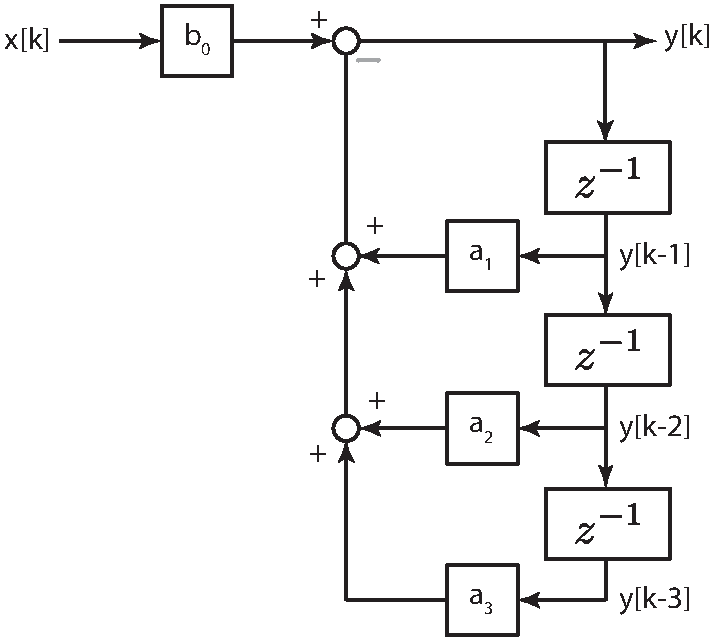
\includegraphics[width=0.7\textwidth]{IIR}
    \caption{Block diagram realization of a third order IIR system
      with static numerator/input dynamics}
        \label{fig:IIR}
\end{figure}

\newpage

\section*{Realization of General Discrete-Time Systems}

Now we will attempt to obtain a realization of more general
discrete-time systems/filters/controllers. Again for the sake
oc clarity let's keep the order (maximum order of $z^{-1}$ in the
equation) of the system to 3. A general third order discrete time
system can be expressed with following difference equation
and transfer function
%
\begin{align*}
y[k] &=  -a_1 y[k-1] - a_2 y[k-2] - a_3 y[k-3] 
+ b_0 x[k] + b_1 x[k-1] + b_2 x[k-2] + b_3 x[k-3] \\ 
Y(z) &= \frac{b_0 + b_1 z^{-1} + b_2 z^{-2} + b_3 z^{-3}}{1+ a_1 z^{-1} + a_2 z^{-2} + a_3 z^{-3}} X(z)
\end{align*}
%
 
\subsection*{Non-minimal Realization / Direct Programming}

One way of realizing a discrete-time system is simply combining
the block diagrams of special cases (i.e. FIR and IIR with static input
dynamics) given in Figures~\ref{fig:FIR} \& \ref{fig:IIR}. The block
diagram realization obtained with this method can be observed in
Fig.~\ref{fig:direct}
%
\begin{figure}[h]
    \centering
      \includegraphics[width=1\textwidth]{direct}
    \caption{Direct/non-minimal realization of a third order discrete
      time dynamical system}
        \label{fig:direct}
\end{figure}

The obvious problem in this realization is that even though the transfer function
represents a third order discrete-dynamical system, the ``order'' 
of the block diagram is indeed 6 not 3. Because there exist 6
different memory blocks, i.e. delay elements. If we forexample
obtain a state-space model from this block diagram we would obtain 
a system with 6 states. 

\newpage

\subsection*{Canonical Realization I / Standard Programming}

In this method of realization, we will use the fact the system is
LTI. Let's consider the transfer function of the system and let's 
perform some LTI operations.
%
\begin{align*}
Y(z) &= \frac{b_0 + b_1 z^{-1} + b_2 z^{-2} + b_3 z^{-3}}{1+ a_1
       z^{-1} + a_2 z^{-2} + a_3 z^{-3}} X(z)
\\
&= \left( b_0 + b_1 z^{-1} + b_2 z^{-2} + b_3 z^{-3} \right) \frac{1}{1+ a_1
       z^{-1} + a_2 z^{-2} + a_3 z^{-3}} X(z) 
\\
&= G_2(z) G_1(z) X(z) \ \mathrm{where} 
\\
G_1(z) &= \frac{H(z)}{X(z)} = \frac{1}{1+ a_1
       z^{-1} + a_2 z^{-2} + a_3 z^{-3}} 
\\
G_2(z) &= \frac{Y(z)}{H(z)} = b_0 + b_1 z^{-1} + b_2 z^{-2} + b_3 z^{-3} 
\end{align*}
%
As you can see we introduced an intermediate variable $h[k]$ with a
Z-transform of $H(z)$, First transfer function, which is an IIR system
with static input dynamics operates on $x[n]$ and produces an output. 
Second transfer function operates on $h[n]$ and produces output
$x[n]$. If we write the difference equations of both systems we obtain
%
\begin{align*}
h[k] &= -a_1 h[y-1] - a_2 h[k-2] - a_3 h[k-3] + x[k] 
\\
y[k] &= b_0 x[k] + b_1 h[k-1] + b_2 h[k-2] + h_3 x[k-3] 
\end{align*}
%
As it can be seen that the delay/shifting operations are only
performed on the signal $h[k]$ and maximum delay operation 
is by 3 samples. Basically if we utilize this structure we can draw a
minimal block diagram representation as given in
Fig.~\ref{fig:standard}. If we obtain a state-space model from this block diagram, the form
will be in \textit{controllable canonical form}. We will cover this
later in the semester. Thus we can call this representation also as 
\textit{controllable canonical realization}. 
%
\begin{figure}[h]
    \centering
      \includegraphics[width=0.55\textwidth]{standard}
    \caption{A minimal block diagram realization of a discrete time
      system obtained with standard programming (Canonical
      representation I)}
        \label{fig:standard}
\end{figure}

\subsection*{Canonical Realization II}

In this method will obtain a different minimal realization. 
The process will be different and this the block diagram will have
different topology. Let's start with the transfer function 
and perform some grouping based on the delay elements.
%
\begin{align*}
&Y(z) ( 1+ a_1 z^{-1} + a_2 z^{-2} + a_3 z^{-3} ) 
= ( b_0 + b_1 z^{-1} + b_2 z^{-2} + b_3 z^{-3} ) X(z)
\\
&Y(z) = b_0 X(z) + z^{-1} \left( b_1 X(z) - a_1 Y(z) \right) + z^{-2} \left( b_2 X(z) -
  a_2 Y(z) \right) + z^{-3} \left( b_3 X(z) - a_3 Y(z) \right)
\\
&Y(z) = b_0 X(z) + z^{-1} \left\lbrace \left( b_1 X(z) - a_1 Y(z) \right) + z^{-1} \left[ \left( b_2 X(z) -
  a_2 Y(z) \right) + z^{-1} \left( b_3 X(z) - a_3 Y(z) \right) \right] \right\rbrace
\end{align*}
%
As you can see we have only $z^{-1}$ terms in the representation there
is a special toplogy embedded inside the expression. If we convert it
to the block diagram form we obtain the structure given in
Fig.~\ref{fig:observable}.
If we obtain a state-space model from this block diagram, the form
will be in \textit{observable canonical form}. Thus we can call this representation also as 
\textit{observable canonical realization}. This form and
representation is the dual of the previous representation. 
%
\begin{figure}[h]
    \centering
      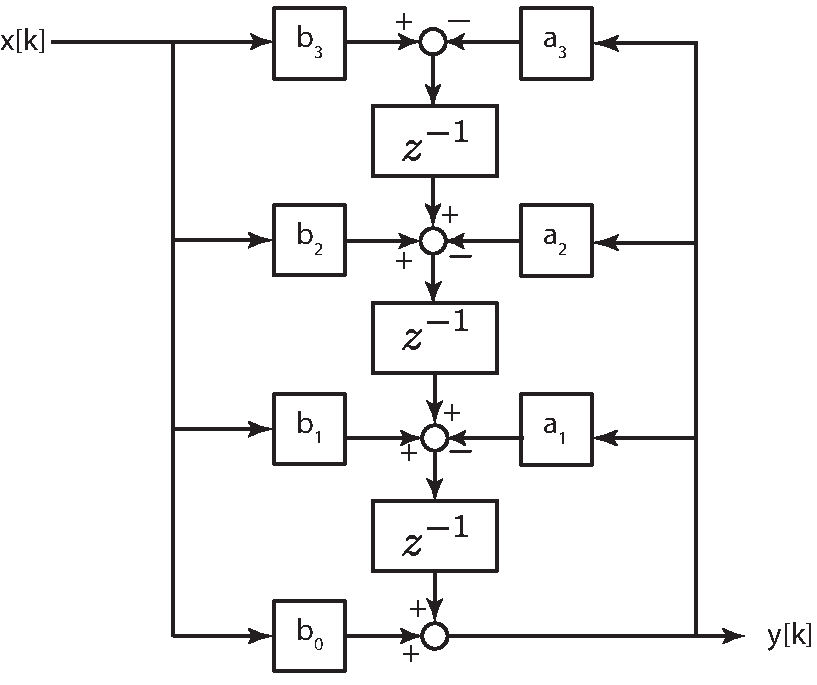
\includegraphics[width=0.75\textwidth]{observable}
    \caption{A minimal block diagram realization of the $3^{rd}$ order
      discrete time system obtained with Canonical representation II}
        \label{fig:observable}
\end{figure}
%

% **** This ENDS THE EXAMPLES. DON'T DELETE THE FOLLOWING LINE:
\end{document}
